\documentclass{beamer}

% Tema y colores
\usetheme{Madrid}
\usecolortheme{whale}

% Paquetes básicos
\usepackage[utf8]{inputenc}
\usepackage[T1]{fontenc}
\usepackage[english]{babel}
\usepackage{graphicx}
\usepackage{hyperref}
\usepackage{amsmath,amsfonts,amssymb}
\usepackage{fancyhdr}
\usepackage{booktabs}
\usepackage{url}
\usepackage{tikz}                % Paquete para gráficos con TikZ
\usetikzlibrary{arrows,positioning}

% Información del título
\title{Machine Learning Final Project}
\subtitle{Custom Implementation of the Apriori Algorithm}
\author{
\begin{tabular}{c} 
Fernanda Flores \\ 
Kevin Arciniegas \\ 
Giussepe Marrero
\end{tabular}
}
\institute{4Geeks Academy}
\date{\today}

\begin{document}

% --- Cover Slide ---
\begin{frame}
    \titlepage
\end{frame}

% --- Table of Contents ---
\begin{frame}{Outline}
    \tableofcontents
\end{frame}

% --- Technical Considerations and Challenges ---
\section{Technical Considerations and \texorpdfstring{$O(2^n)$}{O(2^n)}}

\begin{frame}{1.Technical Considerations and Challenges}
    \begin{itemize}
        \item Mining association rules in large-scale transactional datasets incurs exponential complexity (\(O(2^n)\)).
        \item The standard Apriori algorithm struggles with high-dimensional data due to combinatorial explosion.
        \item Pre-filtering popular products helps reduce the candidate space, theoretically lowering the complexity to \(O(2^{n-3})\) (i.e., reducing cost by a factor of 8).
    \end{itemize}
\end{frame}

% --- Cost Complexity Reduction Illustration ---
\section{Cost Complexity Reduction}

\begin{frame}{2.Cost Complexity Reduction}
    \centering
    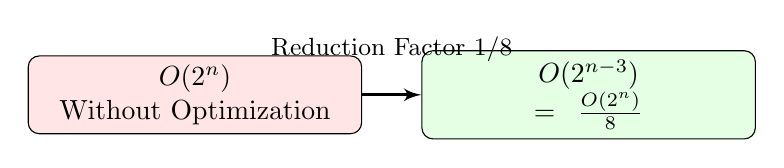
\begin{tikzpicture}[node distance=5cm, auto, >=latex']
        % Nodo original: Complejidad sin optimización
        \node[draw, rectangle, rounded corners, text width=4cm, align=center, fill=red!10] (original) {\(O(2^n)\)\\Without Optimization};
        % Nodo optimizado: Complejidad reducida
        \node[draw, rectangle, rounded corners, text width=4cm, align=center, fill=green!10, right of=original] (optimized) {\(O(2^{n-3})\)\\\(=\frac{O(2^n)}{8}\)};
        % Flecha que indica la reducción
        \draw[->, very thick] (original) -- node[midway, above=8pt]{\small Reduction Factor 1/8} (optimized);
    \end{tikzpicture}
\end{frame}
    

% --- Objectives ---

\section{Objectives}

\begin{frame}{3.Objectives}
    \textbf{General Objective:}
    \begin{itemize}
        \item Develop a functional Apriori algorithm capable of extracting frequent itemsets and generating association rules from transactional data.
    \end{itemize}

    \textbf{Specific Objectives:}
    \begin{itemize}
        \item Implement the modular stages of the Apriori algorithm: candidate generation, pruning, and support calculation.
        \item Address challenges such as data imbalance and ensure compatibility with large-scale datasets.
        \item Evaluate performance metrics such as execution time and memory usage under different dataset conditions.
        \item Document the technical limitations and computational trade-offs encountered during development.
    \end{itemize}
\end{frame}

% --- Description and Analysis of the Dataset ---
\section{Description and Analysis of the Dataset}

\section{Dataset Origin}

\begin{frame}{4.Dataset Origin}
    \begin{itemize}
        \item Relational dataset of Instacart orders, consisting of:
        \begin{itemize}
            \item Over 3 million orders from 200,000+ users.
            \item Each user has 4 to 100 orders.
        \end{itemize}
        \item Dataset is anonymized and publicly available.
        \item \textbf{Source:} \url{https://www.kaggle.com/c/instacart-market-basket-analysis/data}
    \end{itemize}
\end{frame}

\begin{frame}{Dataset Characteristics}
    \begin{itemize}
        \item Focused on two key files for this analysis:
        \begin{itemize}
            \item \textbf{market\_basket\_dataset.csv}: Contains aggregated transactional data for market basket analysis.
            \item \textbf{order\_products\_train.csv}: Includes product IDs and details of purchased items in the training set.
        \end{itemize}
        \item The dataset structure facilitates detailed exploration of customer purchase behaviors and product associations.
    \end{itemize}
\end{frame}


% --- Algorithm Handling: Scope and Limitations ---
\section{Algorithm Handling: Scope and Limitations}

\begin{frame}{5.Algorithm Handling: Scope and Limitations}
    \begin{itemize}
        \item The project leverages a modular approach to implementing the Apriori algorithm, focusing on candidate generation, pruning, and support calculation.
        \item While the algorithm builds upon existing foundations, the emphasis is on adapting it to handle scalability and efficiency challenges.
        \item Modular functions (e.g., pruning based on the Apriori principle) allow for independent testing and debugging of each phase.
        \item Limitations arise primarily from data sparsity, the computational cost of frequent itemset generation, and the efficiency of handling large transaction datasets.
        \item Future optimization could involve incorporating parallelization techniques or integrating more advanced pruning strategies.
    \end{itemize}
\end{frame}

% --- Project Development ---
\section{Project Development}

\begin{frame}{5.Project Development}
    \textbf{Implementation of the Algorithm:}
    \begin{itemize}
        \item Step-by-step development of the Apriori algorithm.
        \item Detailed explanation of candidate reduction mechanisms.
    \end{itemize}
    \vspace{0.5em}
    \textbf{Performance Measurement and Benchmarking:}
    \begin{itemize}
        \item Define performance metrics (e.g., execution time, memory usage).
        \item Comparative analysis against brute-force or alternative approaches.
        \item Presentation of experimental results.
    \end{itemize}
\end{frame}

% --- Metrics ---
\section{Metrics}

\begin{frame}{6.Metrics (Undersampling) for Evaluation}
    \begin{itemize}
        \item Overview of performance metrics used for evaluation.
        \item Explanation of undersampling techniques employed to balance the dataset.
        \item Discussion on how these metrics drive insights for model optimization.
    \end{itemize}
\end{frame}

% --- Conclusions and Business Recommendations ---
\section{7.Conclusions and Business Recommendations}

\begin{frame}{Conclusions and Business Recommendations}
    \begin{itemize}
        \item Summarize key findings and performance analysis.
        \item Discuss the scalability and efficiency of the optimized Apriori implementation.
        \item Provide business recommendations based on the project results.
        \item Suggest potential avenues for future work and improvements.
    \end{itemize}
\end{frame}

% --- References ---
\section{References}

\begin{frame}{8.References}
    \begin{thebibliography}{9}
        \bibitem{agrawal94} R. Agrawal, T. Imielinski, and A. Swami, ``Fast algorithms for mining association rules,'' in \textit{Proc. 20th Int. Conf. Very Large Data Bases (VLDB)}, 1994, pp. 487--499.
        \bibitem{kaggle_instacart} Instacart Market Basket Analysis, Kaggle Competition, [Online]. Available: \url{https://www.kaggle.com/c/instacart-market-basket-analysis/data}. Accessed: Mar. 2025.
        \bibitem{han06} J. Han, M. Kamber, and J. Pei, \textit{Data Mining: Concepts and Techniques}, 2nd ed., Morgan Kaufmann, 2006.
    \end{thebibliography}
\end{frame}

\end{document}


\documentclass{beamer}

% Theme and color settings
\usetheme{Madrid}
\usecolortheme{whale}

% Packages 
\usepackage[utf8]{inputenc}
\usepackage[T1]{fontenc}
\usepackage[english]{babel}
\usepackage{graphicx}
\usepackage{hyperref}
\usepackage{amsmath,amsfonts,amssymb}
\usepackage{fancyhdr}
\usepackage{booktabs}
\usepackage{url}

% Información del título
\title{Machine Learning Final Project}
\subtitle{Custom Implementation of the Apriori Algorithm}
\author{
\begin{tabular}{c} 
Fernanda Flores \\ 
Kevin Arciniegas \\ 
Giussepe Marrero
\end{tabular}
}
\institute{4Geeks Academy}
\date{\today}

\begin{document}

% --- Cover Slide ---
\begin{frame}
    \titlepage
\end{frame}

% --- Table of Contents ---
\begin{frame}{Outline}
    \tableofcontents
\end{frame}

% --- 1. Technical Framework Theory ---
\section{Technical Framework Theory}

\begin{frame}{1. Technical Framework Theory}
    \begin{itemize}
        \item \textbf{Association Rule Mining and Apriori Algorithm:} Identifies \\
              patterns in datasets; Apriori discovers frequent itemsets to extract meaningful rules.
        \item \textbf{Apriori Algorithm Functionality:} Uses a bottom-up approach, \\
              starting with individual items and progressively combining them into larger\\
              itemsets, filtering out infrequent ones based on a minimum support threshold.
        \item \textbf{Computational Challenges:} Faces combinatorial explosion and high \\
              resource demands when processing large datasets.
    \end{itemize}
\end{frame}

% --- 2. Problem Statement ---
\section{Problem Statement}

\begin{frame}{2. Problem Statement}
    \begin{itemize}
        \item There is no efficient method to automatically discover high-quality \\
              association rules in large-scale datasets.
        \item Traditional brute-force approaches become unfeasible due to the combinatorial \\
              explosion of candidate itemsets.
        \item Existing algorithms, including Apriori, struggle with processing high-dimensional\\
              data efficiently.
        \item Optimizing the mining process by pre-filtering popular products and segmenting \\
              orders temporally may improve efficiency and yield actionable insights.
    \end{itemize}
\end{frame}

% --- 3. Project Justification ---
\section{Project Justification}

\begin{frame}{3. Project Justification}
    \begin{itemize}
        \item Current algorithms struggle with combinatorial problems and high resource \\
              consumption.
        \item Implementing Apriori from scratch helps understand its fundamental principles.
        \item Pre-filtering popular products and segmenting orders can improve efficiency \\
              in rule extraction.
        \item The custom approach aims to reduce computational complexity and execution time.
    \end{itemize}
\end{frame}

% --- 4. Objectives ---
\section{Objectives}

\begin{frame}{4. Objectives}
    \textbf{General Objective:}
    \begin{itemize}
        \item Develop an optimized implementation of the Apriori algorithm to efficiently\\
              extract actionable association rules and insights from large-scale datasets.
    \end{itemize}

    \textbf{Specific Objectives:}
    \begin{itemize}
        \item Pre-filter popular products to reduce redundant candidate itemsets and\\
              computational overhead.
        \item Segment transactions based on temporal features (e.g., day of the week or hour) \\
              to uncover context-specific patterns.
        \item Evaluate algorithm performance on large datasets to identify scalability \\
              bottlenecks and potential improvements.
        \item Extract actionable insights into customer purchasing behavior to inform and \\
              enhance future predictive models.
    \end{itemize}
\end{frame}

% --- 5. Description and Analysis of the Dataset ---
\section{Description and Analysis of the Dataset}

\begin{frame}{5.1 Dataset Origin}
    \begin{itemize}
        \item This dataset is a relational set of files describing customers' grocery \\
              orders over time.
        \item It contains over 3 million orders from more than 200,000 Instacart users,\\ 
              with each user having between 4 and 100 orders.
        \item Orders include the sequence of purchased products, order day, hour of placement,\\
              and the relative time between orders.
        \item The dataset is anonymized. For additional details, please refer to the \\
              accompanying blog post.
        \item \textbf{Access the dataset at:} 
        \\\url{https://www.kaggle.com/competitions/instacart-market-basket-analysis/data}
    \end{itemize}
\end{frame}

\begin{frame}{5.2 Dataset Characteristics}
    \begin{itemize}
        \item The dataset is organized into several CSV files, each with unique IDs \\
              and self-explanatory variable names:
        \begin{itemize}
            \item \textbf{aisles.csv}: Lists aisle IDs and names (e.g., "prepared soups salads").
            \item \textbf{departments.csv}: Contains department IDs and names \\
                  (e.g., "frozen", "bakery").
            \item \textbf{order\_products\_\_prior.csv}: Details previous orders, including\\
                  product IDs, add-to-cart order, and a 'reordered' flag.
            \item \textbf{orders.csv}: Identifies order sets (prior, train, test) and provides\\
                  temporal features like day of week and order hour.
            \item \textbf{products.csv}: Lists product IDs, product names, and associated \\
                  aisle and department IDs.
        \end{itemize}
        \item This organization enables detailed analysis of customer purchase behavior.
    \end{itemize}
\end{frame}

% --- 6. Algorithm Handling: Scope and Limitations ---
\section{Algorithm Handling: Scope and Limitations}

\begin{frame}{6. Algorithm Handling: Scope and Limitations}
    \begin{itemize}
        \item Detailed explanation of the Apriori algorithm and its computational cost.
        \item Implementation approach: building the algorithm from scratch.
        \item Pre-filtering popular products and segmenting orders help reduce \\
              redundant candidate itemsets.
        \item Limitations include data size, performance constraints, and combinatorial\\
              challenges.
    \end{itemize}
\end{frame}

% --- 7. Project Development ---
\section{Project Development}

\begin{frame}{7. Project Development}
    \textbf{Implementation of the Algorithm:}
    \begin{itemize}
        \item Step-by-step development of the Apriori algorithm.
        \item Explanation of mechanisms chosen for feature extraction.
    \end{itemize}
    \vspace{0.5em}
    \textbf{Performance Measurement and Benchmarking:}
    \begin{itemize}
        \item Define how performance is measured (execution time, memory usage, etc.).
        \item Comparative analysis: benchmark against brute-force or alternative approaches.
        \item Showcase experiments and results.
    \end{itemize}
\end{frame}

% --- 8. Metrics ---
\section{Metrics}

\begin{frame}{8. Metrics (Undersampling) for Evaluation}
    \begin{itemize}
        \item Description of the performance metrics used for evaluation.
        \item Explanation of undersampling techniques applied to balance the dataset.
        \item How these metrics drive insights for model optimization.
    \end{itemize}
\end{frame}

% --- 9. Conclusions and Business Recommendations ---
\section{Conclusions and Business Recommendations}

\begin{frame}{9. Conclusions and Business Recommendations}
    \begin{itemize}
        \item Summary of key findings and performance analysis.
        \item Discussion on the scalability and efficiency of the custom Apriori implementation.
        \item Business recommendations based on the project outcomes.
        \item Potential avenues for future work and improvements.
    \end{itemize}
\end{frame}

% --- 10. References ---
\section{References}

\begin{frame}{10. References}
    \begin{thebibliography}{9}
        \bibitem{agrawal94} R. Agrawal, T. Imielinski, and A. Swami,
        \\ ``Fast algorithms for mining association rules,'' \\
        in \textit{Proc. 20th Int. Conf. Very Large Data Bases (VLDB)}, 
        \\ 1994, pp. 487--499.
        \bibitem{kaggle_instacart} Instacart Market Basket Analysis, \\
        Kaggle Competition, [Online]. Available:\\
         \url{https://www.kaggle.com/c/instacart-market-basket-analysis/data}.\\
         Accessed: Mar. 2025.
        \bibitem{han06} J. Han, M. Kamber, and J. Pei, \\
        \textit{Data Mining: Concepts and Techniques}, 2nd ed.,
        \\Morgan Kaufmann, 2006.
    \end{thebibliography}
\end{frame}

\end{document}
